\chapter{Semantic Analyses and Typing} \label{chp:semantic-analyses}

When we have successfully obtained a parse AST instance from the previous lexing
and parsing stages, we proceed with semantic analyses, most notably type
inference and type checking of programs.
In this stage, we statically analyse the input program, where SPL's
Hindley-Milner-style type system allows us to catch a large class of errors
at compile time. In particular, we can identify type mismatches, e.g. where
an operator is applied to the wrong argument type, or a field selector is used
with an unsupported type.

Our semantic analyses comprise the following three steps:
\begin{itemize}
  \item In a first step, we \emph{desugar} the parse AST (as given in
        \cref{fig:parse-ast}) to a new AST representation, which we call the
        typing AST; the new AST and desugaring step are described in
        \cref{sec:desugaring}.
  \item Next, we construct the \emph{call graph} of the input program, on which
        we perform a so-called strongly connected components analysis to
        determine how we must group and order the function declarations.
        Further details are given in \cref{sec:scc-analysis}.
  \item Finally, we perform typing inference and type checking on the input
        program. We use the term `typing' to mean both inference and checking,
        as our implementation combines both in one stage.
\end{itemize}


\section{Typing AST and Desugaring} \label{sec:desugaring}

Starting with the program given in the parse AST representation of
\cref{fig:parse-ast}, we proceed by translating the parsed program to a new AST
representation used in the typing stage. \cref{fig:type-ast} shows the data type
declaration for this new \emph{typing AST}.

\paragraph{Functions, operators, and field selectors}
As you can see, the definition for expressions has shrunk somewhat when compared
to the AST of the parsing stage. This is mostly due to the fact that all field
selectors and operators on expressions have been converted to regular function
calls (case \haskell{FunCallE}). Note that we represent function names not
directly as strings/text, but using \haskell{FunName}, which preserves the
distinction between user-defined functions, built-in functions, operators, and
field selectors.
The main reason for grouping all function-like constructs in the
\haskell{FunCallE} node is that we can then treat them more uniformly during the
typing stage.
Also note that field selectors in variable assignments remain unchanged; these
are represented by \haskell{VarLookup}.


\begin{figure}
\begin{minted}[breaklines]{haskell}
data Program varAnn funAnn = Program [VarDecl varAnn] [FunMutDecl varAnn funAnn]
data VarDecl a = VarDecl Loc (Maybe UType) T.Text (Expr a) a
data FunMutDecl a b = MutualDecls Loc [FunDecl a b] | SingleDecl (FunDecl a b)
data FunDecl a b = FunDecl Loc T.Text [T.Text] (Maybe UType) [VarDecl a] [Stmt a] b

data Stmt a = If Loc (Expr a) [Stmt a] [Stmt a]
            | While Loc (Expr a) [Stmt a]
            | Assign Loc VarLookup a (Expr a)
            | FunCall Loc FunName [Expr a]
            | Return Loc (Maybe (Expr a))

data VarLookup = VarId Loc T.Text | VarField Loc VarLookup Field
data Field = Head | Tail | Fst | Snd

data FunName = Name T.Text
             | Not | Neg
             | Add | Sub | Mul | Div | Mod
             | Eq | Neq | Lt | Gt | Lte | Gte
             | And | Or
             | Cons | IsEmpty | Print
             | HeadFun | TailFun | FstFun | SndFun

data Expr a = Ident Loc T.Text a
            | Int Loc Int a
            | Char Loc Char a
            | Bool Loc Bool a
            | FunCallE Loc FunName [Expr a] a
            | EmptyList Loc a
            | Tuple Loc (Expr a) (Expr a) a

type UVar = Int
type TVar = T.Text

data UType = Int | Bool | Char | Void
           | Prod UType UType | List UType | Fun [UType] UType
           | UVar UVar | TVar TVar

data UScheme = UScheme (S.Set UVar) UType
\end{minted}

\caption{Abstract syntax tree representation for typing stage}
\label{fig:type-ast}
\end{figure}


\paragraph{`Garbage' nodes}
In addition, all the garbage nodes available in the parse AST are no longer
present in the typing AST: since the garbage nodes indicate errors in the
parsing stage, we should never proceed to the typing stage in their presence.
Doing so would constitute a compiler bug, hence the desugaring stage includes
sanity checks that throw an error if such nodes are found in the parsed program.

\paragraph{Mutual declarations}
At the top level of the program, the function declarations are now represented
by a list of \haskell{FunMutDecl}, which has two alternatives: either a single
function declaration \haskell{FunDecl} (as in the parsing stage), or a group of
\emph{mutually defined} functions, given instead by a list of \haskell{FunDecl}.
Such groupings of function declarations are needed for handling the strongly
connected components; we defer the details to \cref{sec:scc-analysis}.
For now, we simply convert each \haskell{FunDecl} instance of the parse AST to
a \haskell{SingleDecl} instance in the typing AST.

\paragraph{Type annotation fields}
Another key difference is that we extend many of the nodes with type
parameters \code{a} and \code{b}. The fields correspond to the types we
infer for the respective nodes during the typing stage.
Initially, we have no type information available (aside from the optional type
annotations in the source program), and represent this lack of information
with the \haskell{()} type, e.g. \haskell{Expr ()}. During the typing stage, we
iterate through the typing AST, replacing these dummy fields of type \haskell{()}
with our inferred type information. The type annotations are given by
\haskell{UScheme} for functions, or \haskell{UType} in all other cases.

For instance, when checking an expression $e$, we start with an instance of
\haskell{Expr ()}, and return an instance of \haskell{Expr UType}.
As specified in \cref{fig:type-ast}, the cases for \haskell{UType} match those
in the grammar of SPL types (\cref{chp:grammar}), with the addition of
\emph{unification variables} \haskell{UVar}. These are represented by integers,
and are generated and used as placeholders for unknown types during typing.
A \haskell{UScheme} is just a \haskell{UType}, along with the set of free
unification variables that appear in the type; this corresponds to a polymorphic
type scheme of the form $\forall\ \set{\alpha}.\ \tau$.
Initially, we  annotate each AST node with a unification variable. These are
subsequently replaced once we determine how the placeholders must be
instantiated.

% \todobox{Which nodes feature type information, and which just `thread through' the
% type parameters?}

% \begin{figure}
% \begin{minted}[breaklines]{haskell}
% type UVar = Int
% type TVar = T.Text

% data UType = Int | Bool | Char | Void
%            | Prod UType UType | List UType | Fun [UType] UType
%            | UVar UVar | TVar TVar
% \end{minted}

%   \caption{Algebraic data type of SPL types}
%   \label{fig:type-adt}
% \end{figure}


\section{SCC Analysis} \label{sec:scc-analysis}

In a function declaration---represented by \haskell{FunDecl a b} in the
AST representation of \cref{fig:type-ast}---the body may freely contain function
calls to other functions, or to the function itself.
In the typing algorithm, we must ensure that we process function declarations in
the right order, based on how they reference each other.
If the declaration for some function $f$ refers to a function $g$, we need to
process $g$ first, since we need its type to check that $g$ is used correctly in
the body of $f$.

While we could simply require that the user declare a function before other
functions that reference it, we can also automatically infer this ordering using
the \emph{call graph} of the program.
The call graph has as its vertices the functions declared in the program, while
the edges are given by the function calls between them: if some function $f$
calls the function $g$, this is captured by a directed edge from $f$ to $g$.

\paragraph{Strongly connected components}
There is also the possibility that a function refers to itself
(\emph{recursion}), and---more importantly---that two or more functions refer to
each other in a cycle, in which case they are said to be \emph{mutually
recursive}. We want to identify such groups of functions, since we need some
additional steps in the typing algorithm to handle them correctly.
Again, we can leverage the call graph to find groups of vertices that refer to
each other cyclically; in graph terminology, these are referred to as
\emph{strongly connected components} (SCCs).
Our overall goal is thus to construct the call graph of the input program and
use it to find the SCCs, as well as sorting the (groups of) functions such that
they appear in the output prior to the functions that refer to them.
In graph theory terminology, we want the reverse \emph{topological sorting} of
the directed acyclic graph given by the SCCs of the original call graph.

The so-called strongly connected components algorithm of \citet{Tarjan1972}
lends itself very elegantly to this problem, as it identifies the SCCs of a
directed graph in linear time, while also returning the SCCs in reverse
topological ordering as a by-product.
We do not discuss the inner workings of the algorithm, and our compiler uses an
existing Haskell implementation of Tarjan's algorithm provided in the
\code{Data.Graph} library, based on a Haskell-specific description of
the algorithm due to \citet{King1995}.

\paragraph{Call graph generation}
In order to use the library implementation of the SCC algorithm, we construct
the call graph for the input program in the appropriate format, and then process
the output back into our AST representation, which gives us the sorted program.

The call graph generation is illustrated in \cref{fig:call-graph-example}. The
program outline on the left specifies only the function calls and declarations,
and features the functions \code{p}, \code{f}, \code{g}, \code{h} and
\code{main}.
The call graph corresponding to the program outline is shown on the right.
We identify three strongly connected components: the functions \code{f},
\code{g} and \code{h} refer to each other in a cycle, i.e. their vertices are
all reachable from each other, hence they form an SCC; the remaining functions
\code{p} and \code{main} both constitute a singleton SCC.
The function \code{p} is called by the SCC containing \code{f}, \code{g} and
\code{h}, which in turn is called by \code{main}, hence the sequence of SCCs in
reverse topological ordering is given by:
\[ \langle \{ \code{p} \},\ \{ \code{f}, \code{g}, \code{h} \},\ \{ \code{main} \} \rangle \]

We generate the call graph using the following monad:
\begin{minted}{haskell}
  type GraphGen = StateT GraphGenState (Except T.Text)
\end{minted}
%
Generating the graph requires some auxiliary data structures, which we thread
through the computation using the state monad. The state is given by
\haskell{GraphGenState}\footnote{The actual implementation uses type aliases for
the various map types, which we unfold here.
\haskell{Vertex} is a synonym for \haskell{Int}.}:
\begin{minted}{haskell}
  data GraphGenState = GraphGenState {
    nameMap  :: M.Map T.Text Vertex,
    declMap  :: M.Map Vertex (FunDecl () ()),
    edgeMap  :: M.Map Vertex (S.Set Vertex),
    vtxBound :: Vertex
  }
\end{minted}
%
The \code{nameMap} field associates function identifiers with their respective
vertex ID in the call graph, while \code{declMap} maps the vertices back to the
function declarations, allowing us to easily convert the sorted SCCs back to a
list of (grouped) \haskell{FunDecl}s.
The call graph itself is represented by \code{edgeMap}, which associates each
vertex with the set of its successors. Finally, \code{vtxBound} stores the
largest vertex ID in use, allowing us to generate fresh vertices by incrementing
this number.


\begin{figure}[t]

  \centering

  \begin{minipage}{.45\textwidth}
    \begin{lstlisting}[language=SPL]
      p(x) { $...$ }

      f(x) {
        $...$ g(x,x-1) $...$ p(x) $...$
      }

      g(x,y) {
        $...$ p(y) $...$ h(y) $...$
      }

      h(n) { $...$ f(n/2) $...$ g(n) $...$ }

      main() { $...$ h(f(42)) $...$ }
    \end{lstlisting}
  \end{minipage}\hspace{6mm}%
  %
  \begin{minipage}{.45\textwidth}
    \begin{center}
      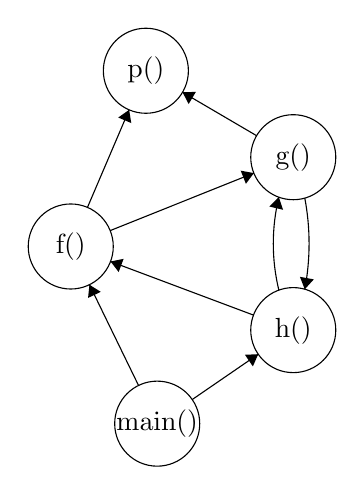
\begin{tikzpicture}[scale=0.18]
        \tikzstyle{every node}+=[inner sep=0pt]
        \draw [black] (33.9,-17.3) circle (3);
        \draw (33.9,-17.3) node { \code{p()} };
        \draw [black] (28.6,-29.7) circle (3);
        \draw (28.6,-29.7) node { \code{f()} };
        \draw [black] (44.3,-23.4) circle (3);
        \draw (44.3,-23.4) node { \code{g()} };
        \draw [black] (44.3,-35.6) circle (3);
        \draw (44.3,-35.6) node { \code{h()} };
        \draw [black] (34.7,-42.2) circle (3);
        \draw (34.7,-42.2) node { \code{main()} };
        \draw [black] (43.284,-32.784) arc (-166.34085:-193.65915:13.905);
        \fill [black] (43.28,-26.22) -- (42.61,-26.88) -- (43.58,-27.11);
        \draw [black] (45.113,-26.284) arc (10.75824:-10.75824:17.23);
        \fill [black] (45.11,-32.72) -- (45.75,-32.02) -- (44.77,-31.84);
        \draw [black] (31.38,-28.58) -- (41.52,-24.52);
        \fill [black] (41.52,-24.52) -- (40.59,-24.35) -- (40.96,-25.28);
        \draw [black] (41.49,-34.54) -- (31.41,-30.76);
        \fill [black] (31.41,-30.76) -- (31.98,-31.5) -- (32.33,-30.57);
        \draw [black] (41.71,-21.88) -- (36.49,-18.82);
        \fill [black] (36.49,-18.82) -- (36.92,-19.65) -- (37.43,-18.79);
        \draw [black] (29.78,-26.94) -- (32.72,-20.06);
        \fill [black] (32.72,-20.06) -- (31.95,-20.6) -- (32.87,-20.99);
        \draw [black] (37.17,-40.5) -- (41.83,-37.3);
        \fill [black] (41.83,-37.3) -- (40.89,-37.34) -- (41.45,-38.16);
        \draw [black] (33.38,-39.5) -- (29.92,-32.4);
        \fill [black] (29.92,-32.4) -- (29.82,-33.33) -- (30.72,-32.9);
      \end{tikzpicture}
    \end{center}
    \vspace{2mm}
  \end{minipage}

  \caption{Example program outline and corresponding call graph}
  \label{fig:call-graph-example}

\end{figure}


In order to build the call graph, we start with the desugared input of type
\haskell{Program () ()}. We then recurse throughout the entire AST
representation to process the function declarations and find all function calls
within those declarations. A function call can appear either as a statement or
in an expression.
When recursing through the AST, we only return a result of the unit type
\haskell{()}; the generated graph is given by the final state under the
\haskell{GraphGen} monad.
Most cases are trivial, as we simply recurse into the subterms (if there are
any). Function declarations are handled as follows:
\begin{minted}{haskell}
  funDeclToGraph :: FunDecl () () -> GraphGen ()
  funDeclToGraph funDecl@(FunDecl _ funName _ _ varDecls stmts _) = do
    declVtx <- nameToVertex funName -- Get existing or new vertex ID
    insertDecl declVtx funDecl -- Map current function's vertex to the declaration
    mapM_ (varDeclToGraph declVtx) varDecls
    mapM_ (stmtToGraph declVtx) stmts
\end{minted}
%
We first get the vertex corresponding to function name. If the function name has
already been encountered, we get the vertex from \code{nameMap}, otherwise we
generate a fresh vertex ID.
We then associate the current declaration with the corresponding vertex ID in
\code{declMap}. In the last two lines, we recurse into the variable declarations
and statements of the function body. Since the output type is always
\haskell{GraphGen ()}, we use \code{mapM\_}, which ignores the result of mapping
the monadic functions onto the lists.

The only other noteworthy case is when we encounter a function call:
\begin{minted}{haskell}
  exprToGraph declVtx (FunCallE _ funName args _) = do
    case funName of
    -- Insert edge for function call
      Name name -> insertEdge declVtx name
      _ -> pure () -- Unless it's a built-in function
    mapM_ (exprToGraph declVtx) args
\end{minted}
%
Here, the first argument is the vertex ID of the current declaration, which is
passed down recursively. We use the vertex ID to insert an edge from the vertex
of the current function to the function that is called, unless \code{funName} is
a built-in function, which we do not include in the SCC analysis.

\paragraph{Processing the SCCs}
The call graph is constructed from the final \code{edgeMap} and \code{declMap}
entries. We store the instances of \haskell{FunDecl} directly in the graph, and
the library function \code{stronglyConnComp} then gives us a list of the sorted
function declaration SCCs, which we convert back to a \haskell{Program} instance
as follows:
\begin{itemize}
  \item For a singleton SCC, we use the \haskell{SingleDecl} constructor;
  \item for a cyclic SCC with one entry (i.e. a recursive function), we
        also generate a \haskell{SingleDecl} node;
  \item for a cyclic SCC containing multiple declarations, we insert a
        \haskell{MutualDecls} node.
\end{itemize}
%
The result is a list of type \haskell{FunMutDecl () ()}, which we combine with
the unchanged list of variable declarations to construct the updated
\haskell{Program} instance.



\section{Typing Stage} \label{sec:typing-stage}

After the desugaring stage and the SCC analysis, our compiler comes to the
typing stage, which does most of the work of the semantic analysis.
In the following, we will briefly talk about scoping in \cref{sec:scoping},
then give a formal account of typing constraints, unification and
substitutions in \cref{sec:unification-substitution}, and then discuss the
machinery used by our implementation of the typing procedure in
\cref{sec:typing-infrastructure}.
From there, we will cover the typing procedure itself in
\cref{sec:typing-procedure}, and finally the annotation of the program AST with
the type information in \cref{sec:elaboration}.



\subsection{Scoping} \label{sec:scoping}
As specified in the grammar given in \cref{chp:grammar}, SPL only allows
variable declarations at the global level, or at the beginning of a function
body. Our implementation thus features two scope levels:
\begin{itemize}
  \item A global scope, which covers top-level variable declarations and all
        function declarations, and
  \item a local scope per function, which features the function arguments and
        the local variables declared at the start of the function body.
\end{itemize}

Consider the following example program:
%
\begin{lstlisting}[language=SPL]
  Int a = 2;

  main(x) :: -> Void {
    Int b = 20;
    print(b * x + a);
    return;
  }
\end{lstlisting}
%
Here, \spl{a} and \spl{f} are bound in the global scope, while \spl{x} and
\spl{b} are bound only in the body of function \spl{f}.

To represent this information, our typing procedure uses two variants of
identifier, as well as two separate environments, one of which stores global
identifiers, while the other tracks local bindings.

\begin{minted}{haskell}
data LocalId = LocalTermVar T.Text | LocalFunName T.Text | RetType
data GlobalId = GlobalTermVar T.Text | GlobalFunName T.Text

data EnvLevel = GlobalLevel | LocalLevel

type GlobalEnv = M.Map GlobalId UScheme
type LocalEnv = M.Map LocalId UType
\end{minted}

The \haskell{LocalId} and \haskell{GlobalId} data types both distinguish between
term variables $x$ and function names $f$ at the respective levels.
\haskell{LocalId} additionally features the special case of \haskell{RetType},
which is used within the local scope of a function body to identify the return
type, as it has no explicit identifier in the source.
Next, we have \haskell{EnvLevel}, which simply serves as a toggle for certain
functions whose behaviour differ depending on the scope.
Finally, \haskell{GlobalEnv} maps \haskell{GlobalId}s to \haskell{UScheme}s,
while \haskell{LocalEnv} maps \haskell{LocalId}s to \haskell{UType}s.
The reason for using \haskell{UScheme} at the top level is that the types of
functions may be generalised in the free unification variables, that is, they
have the general form $\forall\ \set{\alpha}.\ \tau$, while variables are always
assigned monotypes.


\subsection{Type Unification and Substitution} \label{sec:unification-substitution}

During the typing procedure, we generate placeholder type variables (unification
variables) for unknown types. While traversing the program, we identify type
constraints, that is, equalities that must hold between (known or unknown) types.
We write $\tau \sim \sigma$ for the constraint stating that $\tau$ and $\sigma$
must match. For instance, given a function call \code{$f$($e_1$,$...$,$e_n$)}
where $f$ has type $\tau_1\ ...\ \tau_n$ \spl{->} $\tau$ and the expressions
$e_1,\dots,e_n$ have types $\sigma_1,\dots,\sigma_n$, the expression types must
match the input types of $f$, which we express by the constraints $\tau_1 \sim
\sigma_1,\ \dots,\ \tau_n \sim \sigma_n$.

We handle constraints between types by trying to \emph{unify} the left and right
type. Both types may contain placeholder variables for (currently) unknown
types; as such, unification is not just an equality check, but we instead try to
instantiate the unknown variables such that the two types match.
The unification procedure may fail if we cannot find such an instantiation.
If the procedure succeeds, we return a \emph{substitution}, expressing how the
placeholders must be replaced in order to resolve the constraint.

Substitutions $S$ are represented by maps from unification (placeholder)
variables ($\alpha,\beta,\dots$) to types ($\tau,\sigma,\dots$). A type
substitution thus has the general form
$\{ \alpha_1 \mapsto \tau_1, \dots, \alpha_n \mapsto \tau_n \}$.
We write $\tau.S$ for the result of applying the substitution $S$ in the type
$\tau$. This operation is defined as follows:
%
\[
\begin{array}{rcl}
  \alpha.S & \eqdef & S(\alpha) \\
  \Int.S & \eqdef & \Int \\
  \Bool.S & \eqdef & \Bool \\
  \Char.S & \eqdef & \Char \\
  \Void.S & \eqdef & \Void \\
  \TProd{\tau_1}{\tau_2}.S & \eqdef & \TProd{\tau_1.S}{\tau_2.S} \\
  \TList{\tau}.S & \eqdef & \TList{\tau.S} \\
  (\tau_1\ ...\ \tau_n \to \sigma).S & \eqdef & \tau_1.S\ ...\ \tau_n.S \to \sigma.S
  % \Parens{ \TFun{\set{\sigma_i}}{\tau} }.S & \eqdef & \TFun{\set{\sigma_i.S}}{\tau.S}
\end{array}
\]

We further write $S_1 \circ S_2$ for the substitution given by composing $S_1$
after $S_2$, where the composition is defined by:
\[ S_1 \circ S_2 =
    S_1 \circ \{ \alpha_1 \mapsto \tau_1, \dots, \alpha_n \mapsto \tau_n \} \eqdef
    \{ \alpha_1 \mapsto \tau_1.S_1, \dots, \alpha_n \mapsto \tau_n.S_1 \} \cup S_1 \]
%
That is, applying the composed substitution $S_1 \circ S_2$ is equivalent to
applying $S_2$ followed by $S_1$.
\[ \tau.(S_1 \circ S_2) = \tau.S_2.S_1 \]

During the unification procedure, we need to determine the set of (free)
placeholder type variables in a given type $\tau$.
We denote this set of free variables with $\FV(\tau)$, where the function
$\FV$ is defined by:
%
\[
\begin{array}{rcl}
  \FV(\alpha) & \eqdef & \{ \alpha \} \\
  \FV(\tau) & \eqdef & \emptyset, \text{ if } \tau \in \{\Int,\Bool,\Char,\Void\} \\
  % \FV(\Bool) & \eqdef & \emptyset \\
  % \FV(\Char) & \eqdef & \emptyset \\
  % \FV(\Void) & \eqdef & \emptyset \\
  \FV( \TProd{\tau_1}{\tau_2} ) & \eqdef & \FV(\tau_1) \cup \FV(\tau_2) \\
  \FV( \TList{\tau} ) & \eqdef & \FV(\tau) \\
  \FV( \tau_1\ ...\ \tau_n \to \sigma ) & \eqdef &
    \FV(\tau_1) \cup \dots \cup \FV(\tau_n) \cup \FV(\sigma)
\end{array}
\]

With the notion of substitutions and the function $\FV$ in place, we define
the unification procedure. The function $\unify$ takes two types and attempts to
unify them, resulting either in a failure $\textsf{Fail}$, or some substitution
$S$. We denote the empty substitution by $\emptyset$.
%
\[
\begin{array}{rcl}
  \unify(\tau,\tau) & \eqdef & \emptyset, \text{ if } \tau \in \{\Int,\Bool,\Char,\Void\} \\
  % \unify(\Int,\Int) & \eqdef & \emptyset \\
  % \unify(\Bool,\Bool) & \eqdef & \emptyset \\
  % \unify(\Char,\Char) & \eqdef & \emptyset \\
  % \unify(\Void,\Void) & \eqdef & \emptyset \\
  \unify(\alpha,\alpha) & \eqdef & \emptyset \\
  \unify(\alpha,\tau) & \eqdef &
    \{ \alpha \mapsto \tau \},\ \text{if}\ \alpha \notin \FV(\tau) \\
  \unify(\tau,\alpha) & \eqdef & \unify(\alpha,\tau) \\
  \unify(\TList{\tau},\TList{\sigma}) & \eqdef & \unify(\tau,\sigma) \\
  \unify(\TProd{\tau_1}{\tau_2}, \TProd{\sigma_1}{\sigma_2}) & \eqdef &
    \unify( \tau_2.S, \sigma_2.S ) \circ S,
    \text{ where } S = \unify(\tau_1,\sigma_1)
\end{array}
\]

In the third case, the side condition $\alpha \notin \FV(\tau)$ is the so-called
\emph{occurs check}, stating that we cannot unify $\alpha$ with a larger type
that (freely) features $\alpha$ as a subterm.
For instance, we cannot solve the constraint $\alpha \sim \TProd{\alpha}{\Int}$,
since this constraint can only be solved by an infinite type\footnote{%
We return to the topic of infinite types and how our extension adds support for
them in \cref{sec:ext-syntax-features}}.

We lift $\unify$ to (possibly empty) sequences of types, which we denote using
the overlined notation of \citet{Igarashi2001} as $\set{\tau_i}$. The
unification of sequences of types is defined recursively by:
\[ \unify(\tau\ \set{\tau_i},\ \sigma\ \set{\sigma_i}) \eqdef
    \unify(\set{\tau_i.S},\ \set{\sigma_i.S}) \circ S,
    \text{ where } S = \unify(\tau,\sigma) \]
If both sequences are empty, the result is the empty substitution $\emptyset$.

The above allows us to define unification for function types as follows:
\[ \unify(\set{\tau_i} \to \tau,\ \set{\sigma_i} \to \sigma) \eqdef
    \unify(\tau.S,\sigma.S) \circ S, \text{ where } S = \unify(\set{\tau_i}, \set{\sigma_i}) \]

For all other combinations of types $\tau$ and $\sigma$ not covered by the
equations above, the types cannot be unified and the result of
$\unify(\tau,\sigma)$ is `\textsf{Fail}'.

\paragraph{Example}
To illustrate, let us consider how we determine the type of the
expression \spl{(1,True).fst}. The field selector \spl{.fst} is represented by a
function call, meaning we can think of the expression as something
closer to \spl{fstfun((1,True))}. The type of \spl{fstfun} is polymorphic, and
given by the type scheme $\forall \alpha \beta.\ \code{(}\alpha,\beta\code{)}
\to \alpha$, expressing that \spl{fstfun} returns the first/left entry with type
$\alpha$.

During typing, we instantiate the type variables $\alpha$ and $\beta$ in the
type scheme $\forall \alpha \beta.\ \code{(}\alpha,\beta\code{)} \to \alpha$
with placeholder unification variables, for which we write $u_1$ and $u_2$.
We then have \spl{($u_1$,$u_2$)} as the placeholder for the input type
\spl{fstfun}, while $u_2$ is also the placeholder for the output, and thus also
the placeholder for the type of the expression \spl{(1,True).fst}.

For the pair former \spl{($-$,$-$)}, the type is given by the two inner types,
i.e. the types of \spl{1} and \spl{True}, which are trivial to determine, and do
not yield any constraints or substitutions.
Having found that \spl{(1,true)} has type \spl{(Int,Bool)}, we return
to the constraints from earlier:
We now have the constraint \spl{($u_1$,$u_2$)} $\sim$ \spl{(Int,Bool)}, where
applying unification with
$\unify($\spl{($u_1$,$u_2$)},\spl{(Int,Bool)}$)$ succeeds, and returns the
substitution $\{ u_1 \mapsto \text{\spl{Int}}, u_2 \mapsto \text{\spl{Bool}} \}$.
Applying the substitution to the placeholder type $u_1$ for \spl{(1,True).fst},
we find that the type of the expression is \spl{Int}.




\subsection{Code Infrastructure} \label{sec:typing-infrastructure}

We represent substitutions as finite maps from \haskell{UVar} to types
\haskell{UType}:
\begin{minted}{haskell}
  newtype Subst = Subst (M.Map UVar UType)
\end{minted}

Composition of substitutions is defined via an instance of Haskell's
\haskell{Monoid} typeclass, where the binary operation is defined as composition
$S_1 \circ S_2$, and the unit element is the empty substitution $\emptyset$:
%
\begin{minted}{haskell}
instance Semigroup Subst where
  Subst s1 <> Subst s2 = Subst $ M.map (subst (Subst s1)) s2 `M.union` s1

instance Monoid Subst where
  mempty = Subst M.empty
\end{minted}

When applying substitutions or determining the free variables, we want to work
interchangeably with \haskell{UType} and \haskell{UScheme}. We achieve this by
defining the following typeclass, of which we declare instances for both
\haskell{UType} and \haskell{UScheme}:
\begin{minted}{haskell}
  class Types a where
    subst :: Subst -> a -> a
    freeUVars :: a -> S.Set UVar
\end{minted}
%
The functions are implemented according to the definitions in
\cref{sec:unification-substitution}.

Our typing monad is defined as follows:
\begin{minted}{haskell}
  data CGenState = CGenState{
    globalEnv :: GlobalEnv,
    localEnv :: LocalEnv,
    varState :: UVar
  }
  type CGen = StateT CGenState (Except T.Text)
\end{minted}

The first two entries represent the global and local environment, as discussed
in \cref{sec:scoping}. For the sake of simplicity, we track the local
environment in the state monad and simply reset it once we have finished
processing a function declaration.
Whenever we obtain new information from unifying types, we apply the resulting
substitution to the local and global environment, replacing any placeholder
variables for which we have found the concrete instantiation.

The third entry lets us generate fresh variable names: since \haskell{UVar} is
just an alias for \haskell{Int}, we can obtain a fresh unification variable by
reading and incrementing the (strictly increasing) value of \code{varState}.

Since we carried over the location data from the parse AST to the various nodes
of the typing AST, we can provide the user with localised type errors using the
\haskell{Except} monad in the \haskell{CGen} monad stack:
\begin{minted}{haskell}
  throwLocError :: Loc -> T.Text -> CGen a
  throwLocError loc msg = throwError $ T.pack (locPretty loc) <> ":\n" <> msg
\end{minted}
%
The helper function \code{locPretty} prints the file path, followed by the line
and column range of the node where the error was encountered.


\subsection{Typing Procedure} \label{sec:typing-procedure}

We now present our typing procedure. By misuse of notation, we describe
the cases of the algorithm in deduction rules, where the judgement
$\Gamma \vdash_W e : \tau, S$ states that in context $\Gamma$, the expression $e$
is typed with $\tau$ under generation of the substitution $S$.
When considering a list of expressions, such as the arguments to a function, we
again use the overlined notation $\set{e_i}$ for a (possibly empty) sequence
$e_1,\dots,e_n$. We also extend this notation to types, substitutions and the
typing judgement, as seen in e.g. \ruleref{W-FunCall}, where the judgement
\[ \set{ \Gamma \vdash_W e_i : \tau_i,\ S_i } \]
states that in context $\Gamma$, the $i$-th expression $e_i$ has type $\tau_i$,
generating the substitution $S_i$.
We further write $\set{S_i}$ to mean the composition of all $S_i$ in order, that
is, $S_n \circ \dots \circ S_1$.
%
The judgement $\fresh(\alpha)$ states that the unification variable $\alpha$ is
freshly generated.
We write $\inst(\forall\ \set{\alpha}.\ \tau)$ for the type $\tau$ in which
all $\set{\alpha}$ have been substituted with fresh unification variables.

\begin{figure}[b]
  \begin{mathpar}

    \inferrule[W-Var]
      {\Gamma(x) = \tau}
      {\Gamma \vdash_W x : \tau,\ \emptyset}

    \inferrule[W-Int]{ }
      {\Gamma \vdash_W n : \code{Int},\ \emptyset}

    \inferrule[W-Bool]{ }
      {\Gamma \vdash_W b : \code{Bool},\ \emptyset}

    \inferrule[W-Char]{ }
      {\Gamma \vdash_W c : \code{Char},\ \emptyset}

    \inferrule[W-Empty]%
      {\fresh(\alpha)}
      {\Gamma \vdash_W \code{[]} : \code{[$\alpha$]},\ \emptyset}

    \inferrule[W-Tuple]%
      {\Gamma \vdash_W e_1 : \tau_1,\ S_1 \\
      \Gamma \vdash_W e_2 : \tau_2,\ S_2}
      {\Gamma \vdash_W \code{($e_1$,$e_2$)} : \code{($\tau_1$,$\tau_2$)},\ S_2 \circ S_1}

    \inferH{W-FunCall}%
      {\mathit{inst}(\Gamma(f)) = \set{\sigma_i} \to \sigma \\
        \set{ \Gamma \vdash_W e_i : \tau_i,\ S_i} \\
        S = \unify(\set{\sigma_i, \tau_i})}
      {\Gamma \vdash_W \code{$f$($\set{e_i}$)} : \tau.S,\ S \circ \set{S_i}}
  \end{mathpar}

  \caption{Rules for the type inference algorithm on expressions}
  \label{fig:typing-rules-expr}
\end{figure}

\paragraph{Expressions}
In \cref{fig:typing-rules-expr}, we describe the cases of the typing procedure
for expressions.
The most important case is \ruleref{W-FunCall}, which subsumes the application
of built-in and user-defined functions as well as field selectors, thanks to our
uniform treatment of the aforementioned constructs (as discussed in \cref{sec:desugaring}).
We look up the function $f$ in the environment $\Gamma$, which (if $f$ has been
declared) yields a type scheme of the form $\forall\ \set{\alpha_j}.\ \tau$.
Next, we instantiate the typing scheme with fresh placeholder variables, i.e.
we substitute each $\alpha_j$ with some fresh $u_j$ in $\tau$, resulting in the
function type $\set{\sigma_i} \to \sigma$.

Note that the length of the sequence $\set{\sigma_i}$ must match that of
$\set{e_i}$ (as indicated by the use of $i$ for both).
We type all the arguments $e_i$, yielding the types $\tau_i$ and the
substitutions $S_i$. We then unify the input types $\set{\sigma_i}$ of the
function with the argument types $\set{\tau_i}$, resulting in the substitution
$S$. Finally, the type of the function call $f\code{($\set{e_i}$)}$ is given by
$\tau.S$, and we return the substitution $S \circ \set{S_i}$.

In the rule above, we write $\Gamma(f)$ for looking up the type of $f$, but in
practice, we only look up $f$ in the context if it is a user-defined function,
and otherwise we simply return a hard-coded type scheme:
\begin{minted}{haskell}
  getFunType :: FunName -> Loc -> CGen UScheme
  getFunType (Name name) loc = do
      mFunType <- envLookupFun name
      case mFunType of
        Nothing -> throwLocError loc $ "No declaration for function `" <> name <> "`"
        Just funType -> pure funType
  getFunType Not _ = pure $ UScheme S.empty (Fun [Bool] Bool)
  getFunType Neg _ = pure $ UScheme S.empty (Fun [Int] Int)
  ...
\end{minted}
%
The type schemes for the operators \spl{Not}, \spl{Neg}, etc are of course all
monomorphic, hence the set of type variables in the type scheme is empty.
More specifically, the types specified above correspond to
\[\begin{array}{rcl}
  \code{Neg} & : & \forall\ .\ \text{\spl{Bool -> Bool}} \\
  \code{Not} & : & \forall\ .\ \text{\spl{Int -> Int}}
\end{array}\]
%
The types for the built-in functions and field selectors are also hard-coded,
for instance:
\[\begin{array}{rcl}
  \code{Cons}    & : & \forall\ \alpha .\ \text{\spl{$\alpha$ [$\alpha$] -> [$\alpha$]}} \\
  \code{IsEmpty} & : & \forall\ \alpha .\ \text{\spl{[$\alpha$] -> Bool}} \\
  \code{HeadFun} & : & \forall\ \alpha .\ \text{\spl{[$\alpha$] -> $\ \alpha$}} \\
  \code{FstFun}  & : & \forall\ \alpha, \beta .\ \text{\spl{($\alpha$,$\beta$) -> $\ \alpha$}}
\end{array}\]

\paragraph{Statements}
Statements are handled in largely the same way as expressions, except that they
do not have a type, so we use the rule format $\Gamma \vdash_W s, S$.
The while-case can be described as follows:
%
\begin{mathpar}
  \inferH{W-While}%
    { \Gamma \vdash_W e : \tau.\ S \\
      \set{ \Gamma \vdash s_i.\ S_i } \\
      S' = \unify(\tau,\Bool) }
    { \Gamma \vdash_W \code{while}\ e\ \code{\{}\ \set{s_i}\ \code{\}},\
      \set{S_i} \circ S' \circ S }
\end{mathpar}
%
We discuss the remaining cases informally:
If-else-statements are just a slight variation on \ruleref{W-While} above, and
function calls are handled exactly the same as in \ruleref{W-FunCall}.
For return statements, we look up the return type of the surrounding function
declaration, which is stored in the local environment, and then either unify it
with the type of $e$ for \spl{return $\ e$;}, or with $\Void$ for \spl{return;}.

Variable assignments are arguably the most interesting case. We start by typing
the expression $e$ on the left, and then we iterate through the sequence of
field selectors from left to right, adjusting the type of the expression in each
step. For instance, in the assignment \spl{x.fst.hd = 1;}, we start with the type
\spl{Int} of \spl{1}, and based on the rightmost selector \spl{.hd}, we adjust
the type to \spl{[Int]}. For \spl{.fst}, we then adjust the type to
\spl{([Int],$u$)}, where $u$ is some fresh placeholder variable.


\paragraph{Declarations}
So far, we have seen how the types of variables and functions are looked up in
the environment, but we also need to insert these types into the environment,
which happens when we process variable and function declarations.

Variable declarations are rather straightforward: we determine the type of the
left-hand side expression, which we unify with the type of the variable (if a
type is specified).
We then update either the local or global environment to map the variable name
to its type.

For function declarations, we generate fresh placeholder variables for the
argument types and return type, which we associate to the parameter names and
the \haskell{RetType} variant in the local environment.
We also use an entry for the function itself in the local environment, such that
we can correctly handle recursive function calls.
Next, we process the variable declarations and statements of the function body.

Aside from handling the constraints that arise from the body of the function, we
also want to check our inferred function type against the type annotation
provided by the user.
Much like instantiating typing schemes with $\mathit{inst}$ in
\ruleref{W-FunCall}, we must instantiate the type variables in the annotated
type with fresh placeholder variables:
\begin{minted}[linenos]{haskell}
  instantiateUserType :: UType -> CGen UType
  instantiateUserType ty = do
    let tVars = freeTVars ty
    s <- sequence $ M.fromSet (const freshVar) tVars
    pure $ substTVars s ty
\end{minted}
%
On line 3, we determine the set of free type variables in the annotated type.
Note that in our inferred types, the type variables are \haskell{UVar}s,
represented by integers, while in the user type annotations, they are
\haskell{TVar}s, represented by \haskell{Text}.
On line 4, we generate a substitution mapping each of the type variables to a
fresh placeholder variable. We then apply the substitution and return the result
(line 5).

Finally, we combine all the substitutions arising from the function body and
unification with the user-specified type and apply the result to the function
type we generated at the beginning. We then associate the resulting type scheme
to the function name in the global environment.

\paragraph{Mutual declarations}
Function declarations that are mutually defined (i.e. mutually recursive) are
already grouped in a \haskell{MutualDecls} node thanks to the SCC analysis
discussed in \cref{sec:scc-analysis}.
When dealing with mutually recursive functions, we must take care to not
generalise too eagerly.
In particular, we first generate placeholder type schemes for all functions in
the SCC, which we insert into the environment (we will update the types later).
We then process all function declarations in order, resulting in a combined
substitution $S$. We go back over the function declarations, applying the $S$ to
each of them.
Only then do we generalise all the type schemes and insert them into the
environment again, updating the original placeholder type schemes.

To give an example, consider the following two mutually recursive functions that
determine whether the length of a list is even (resp. odd):

\begin{center}
\begin{minipage}{.4\textwidth}
  \centering
\begin{lstlisting}[language=SPL]
  lenEven(l) :: [a] -> Bool {
    if (isEmpty(l)) {
      return True;
    } else {
      return lenOdd(l.tl);
    }
  }
\end{lstlisting}
\end{minipage}\hspace{8mm}%
\begin{minipage}{.4\textwidth}
  \centering
\begin{lstlisting}[language=SPL]
  lenOdd(l) :: [a] -> Bool {
    if (isEmpty(l)) {
      return False;
    } else {
      return lenEven(l.tl);
    }
  }
\end{lstlisting}
\end{minipage}
\end{center}\vspace{2mm}

In the recursive case, the functions call each other with the tail of the list
\spl{l}, hence the type parameters of the two functions need to match.
While typing \spl{lenEven}, we find that its input type must be instantiated to
that of \spl{lenOdd}, but the type of \spl{lenOdd} is at that point still a
placeholder type.
While processing \spl{lenOdd}, we substitute the placeholder input type with
some list type \spl{[$\alpha$]}, which then no longer matches the input type we
determined for \spl{lenEven}. We thus need to go back and perform the same
substitution in the type of \spl{lenOdd}, after which the input types match
again.


\subsection{Elaboration} \label{sec:elaboration}

During the typing procedure, we update the local and global environment whenever
we find new information, applying the substitutions that arise from the program.
We do not, however, update the type annotation fields in the AST nodes as we go,
meaning that these still contain the placeholder variables, rather than the
final types we inferred for them.

The type fields thus need to updated throughout the AST using the full
substitution that was returned by the typing procedure; we refer to this step as
\emph{elaboration}.
In essence, we just recurse through the AST, applying the substitution to type
labels wherever they appear in the nodes.
For literal expressions, we include sanity checks for the case that they have
some unexpected type, which would suggest an implementation error:
\begin{minted}{haskell}
  annotateExpr :: Subst -> T.Expr UType -> T.Expr UType
  annotateExpr s (T.Ident loc name ty) = T.Ident loc name (subst s ty)
  annotateExpr _ e@(T.Int loc n Int) = e
  annotateExpr _ (T.Int _ _ ty) = error $ "Integer has type " ++ show ty
  ...
  annotateExpr s (T.FunCallE loc funName args ty) =
    T.FunCallE loc funName (annotateExpr s <$> args) (subst s ty)
  annotateExpr s (T.EmptyList loc ty) =
    T.EmptyList loc (subst s ty)
  annotateExpr s (T.Tuple loc e1 e2 ty) =
    T.Tuple loc (annotateExpr s e1) (annotateExpr s e2) (subst s ty)
\end{minted}

Updating all the type labels allows us to pretty-print the AST with all the type
annotations, which is helpful for debugging purposes.
More importantly though, we require the type annotations to resolve the
overloading of the built-in printing and comparison functions during code
generation, as covered in the following chapter.
